% $Date: 2022/12/30 17:24:03 $
% This template file is public domain.
%
% TUGboat class documentation is at:
%   http://mirrors.ctan.org/macros/latex/contrib/tugboat/ltubguid.pdf
% or
%   texdoc tugboat

\documentclass[final]{ltugboat}

\usepackage{amsmath}
\usepackage{microtype}
\usepackage{graphicx}
\usepackage[hidelinks,pdfa]{hyperref}
\usepackage{hologo}
\usepackage{fontawesome}
\usepackage{ragged2e}
\makeatletter
%listings float without package
\newenvironment{listing*}{\@dblfloat{listing}}{\end@dblfloat}
\def\ext@listing{lol}
\newcommand*{\ftype@listing}{4}
\newcounter{listing}
\newcommand*{\fnum@listing}{\textbf{Listing~\thelisting}}
\def\fps@listing{p}
\makeatother
\usepackage{fancyvrb,fvextra}
\fvset{breaklines}
\usepackage{tikz}
\usetikzlibrary{calc,decorations.pathreplacing,shapes}
\usepackage{./examples}
\def\url{\tbsurl}
\def\AllTeX{(\La\kern-.075em)\kern-.075em\TeX}

%%% Start of metadata %%%
\title{Fast Regression Testing of \TeX{} Packages: The Unreasonable Effectiveness of Batching}

% repeat info for each author; comment out items that don't apply.
\author{Vít Starý Novotný}
\address{Studená 453/15 \\ Brno, 63800 \\ Czech Republic}
\netaddress{witiko (at) mail dot muni dot cz}
\personalURL{github.com/witiko}

\author{Marei Peischl}
\address{Gneisenaustr. 18 \\ Hamburg, 20253 \\ Germany}
\netaddress{marei (at) peitex dot de}
\personalURL{peitex.de}

%%% End of metadata %%%

\begin{document}
\maketitle

\begin{abstract}
Small \TeX{} packages, often created for one-time use, usually depend on user feedback to maintain code quality. However, this approach has its limitations. Larger projects, especially those that are continuously developed, require a more robust solution. Automated regression tests are crucial in these cases. They ensure that any changes, either in the code itself or its external dependencies, do not alter the expected behavior of the code. This helps in maintaining the integrity of the project over time.

In version 3.0.0 of the Markdown package for \TeX, the number of tests increased from 143 to 783. This caused the tests to run for up to 15~hours, which slowed down our development cycle.
In this article, we describe a novel technique for batching test files that reduced our testing time from 15 hours to just 15 minutes. We also discuss how our technique can speed up other regression testing frameworks for \TeX{} packages such as l3build.
Our discussion is aimed at encouraging more efficient testing methods in the broader community of \TeX{} enthusiasts.
\end{abstract}

\section{Introduction}
The Markdown package for \TeX{} features a series of regression tests, enabling developers to ensure that their modifications do not negatively impact existing functionality. These tests, designed to be completed in just a few minutes, provide immediate feedback and are automatically conducted on any updates submitted to the package's GitHub repository.

After the implementation of the CommonMark standard in version 3.0.0 of the Markdown package, the number of tests increased from 143 to 783 (about 5.5 times). This had caused the tests to run for up to 15 hours using free GitHub-hosted runners, which was too slow to provide any benefit to developers.

In order to increase the testing speed, we implemented a novel technique for batching test files and we added self-hosted runners with up to 12 \acro{CPU}s. After these changes, the tests finish in about 15 minutes, which is a 60-fold speed increase and which makes the tests practically useful to developers.

In this article, we describe the testing framework of the Markdown package. In sections~\ref{sec:on-disk-files} and \ref{sec:techniques}, we describe the on-disk files and techniques used in our framework. In Section~\ref{sec:implementation}, we describe our implementation. In sections~\ref{sec:experiments} and \ref{sec:results}, we describe our experiments and their results. In Section~\ref{sec:related-work}, we discuss prior work related to our framework. We conclude in Section~\ref{sec:conclusion} by summarizing our contributions and outlining future work.

\section{On-disk files}
\label{sec:on-disk-files}

\looseness=-1
In this section, we describe the on-disk files used in our framework: test files, formats, commands, and templates. We also show how we use them for testing.

\subsection{Test files}
\label{sec:test-files}

\looseness=-1
The Markdown package converts markdown text to \TeX{} commands. To validate the conversion, our framework redefines these \TeX{} commands to produce output in the \texttt{.log} file, which we can examine.

A \emph{test file} consists of a) \TeX{} code that configures the Markdown package, b) markdown text, and c) the expected output in the \texttt{.log} file.

See example test file \file{strike-through.test}, which tests the strike-through syntax extension:

\smallskip
\noindent
\example*[\input images/strike-through.tex]{strike-through.test}

\subsection{Formats, commands, and templates}
\label{sec:formats-commands-and-templates}

\looseness=-1
The Markdown package supports several combinations of \TeX{} formats and engines. For each \TeX{} format, there are also several ways to input markdown text. Our framework ensures that a markdown text always produces the same output.

A \emph{format} consists of one or more a) \emph{commands} that can be used to typeset documents in a \TeX{} format using different \TeX{} engines and b) \emph{templates} that specify the different ways in which markdown text can be input with the \TeX{} format.

Here is an example format \texttt{plain} with commands for the \hologo{pdfTeX}, \Hologo{XeTeX}, and \Hologo{LuaTeX} engines:

\smallskip
\noindent
\addtocounter{footnote}{1}%
\footnotetext{%
  The Markdown package uses Lua to parse markdown text. Whereas Lua\TeX{} can execute Lua code directly, other \TeX{} engines must use the shell of the operating system to execute Lua code. Since accessing the shell is a security risk, users must express their consent by writing \texttt{--shell-escape}.%
}%
\example[%
  \addtocounter{footnote}{-2}%
  \fvset{commandchars=\\\{\}}%
]{COMMANDS.m4}

\smallskip
\noindent
The format \texttt{plain} also contains two templates. One uses the \cs{markdownInput} \TeX{} macro and the other one uses the \cs{markdownBegin} and \texttt{End} \TeX{} macros:

\smallskip
\noindent
\example{input.tex.m4}

\smallskip
\exampleSeparator

\smallskip
\noindent
\example[\fvset{commandchars=|<>}]{verbatim.tex.m4}

\subsection{Materialized templates and commands}
\label{sec:materialized-templates-and-commands}

During testing, the texts \texttt{TEST\_SETUP\_FILENAME} and \texttt{TEST\_INPUT\_FILENAME} in a template are replaced with names of files that contain the \TeX{} code and the markdown text parts of a test file, respectively. Additionally, the text \texttt{undivert(TEST\_INPUT\_FILENAME)} is replaced with the literal markdown text from the test file. After the replacement, we say that the template has been \emph{materialized}.

Here is the template \file{verbatim.tex.m4} from Section~\ref{sec:formats-commands-and-templates} after it has been materialized with the test file \file{strike-through.test} from Section~\ref{sec:test-files}:

\smallskip
\noindent
\combineFiles{verbatim.tex.m4}{strike-through.test} \\[0.4em]
\example{verbatim.tex}

\smallskip
\exampleSeparator

\smallskip
\noindent
\example{test-setup.tex}

\smallskip

After a template has been materialized, the text \texttt{TEST\_FILENAME} in a command is replaced with the filename of the materialized template. After the replacement, the command has also been materialized.

Here are the commands \file{COMMANDS.m4} from Section~\ref{sec:formats-commands-and-templates} after they have been materialized:

\smallskip
\noindent
\combineFiles{COMMANDS.m4}{verbatim.tex} \\[0.8em]
\example{COMMANDS}

\smallskip

\noindent
During testing, the materialized commands are executed. Each command produces a \texttt{.log} file, which is compared to the expected output from the test file.

\section{Techniques}
\label{sec:techniques}
In this section, we describe the computational techniques of multiprocessing and the batching of test files. We also show how we use these techniques to increase the speed of testing in our framework.

\subsection{Multiprocessing}
\label{sec:multiprocessing}
Whereas \TeX{} only uses a single \acro{CPU}, modern computers contain several \acro{CPU}s. Therefore, we can increase the speed of testing by using \emph{multiprocessing}, where each \acro{CPU} processes a different test file:\footnote{%
The image depicts a \acro{CPU} as a \acro{PC}, offering a streamlined perspective. In reality, although most \acro{PC}s have one \acro{CPU}, modern \acro{CPU}s include multiple logical cores, each functioning as a separate \acro{CPU}. For instance, a \acro{PC} with an AMD Ryzen 9 5950X \acro{CPU} has 32 logical cores. With multiprocessing, we can use these cores to increase the testing speed up to 32 times.%
\looseness=-1
}

\smallskip
\noindent
\begingroup
\centering
\input images/server-loaded.tex
\par
\endgroup

\smallskip
\noindent
Using $N$ \acro{CPU}s increases testing speed up to $N$ times.

\subsection{Batching of test files}
\label{sec:batching-of-test-files}
At the beginning of a \TeX{} document, \TeX{} packages, fonts, Lua scripts, and other assets are initialized, which slows down testing:

\smallskip
\noindent
\example*[\input images/verbatim.tex]{verbatim.tex}

\smallskip

To increase the speed of testing, we can amortize the cost of initialization by materializing a template with a \emph{batch} of several test files:

\medskip
\noindent
\combineFiles{input.tex.m4}{first.test, second.test, third.test} \\
\example{input.tex}

\smallskip
\noindent
Batching $N$ test files decreases initialization cost $N$ times. How much this speeds up testing depends on the ratio between the time spent on initialization and the time spent on processing the rest of the template.

If tests use a lot of memory that is not immediately freed, using multiprocessing and batching increases the memory footprint of testing. Specifically, using $M$ \acro{CPU}s and batching $N$ test files increases the memory footprint of testing up to $M\cdot N$ times.

\begin{listing*}
\bigExample*[\input images/test.tex]{test.sh}
\caption{The shell script \file{test.sh} that implemented the testing framework of the Markdown package before version 3.0.0. For each test file, \file{test.sh} a) materializes templates in a temporary directory, b) executes the materialized commands, and \linebreak c) compares the \texttt{.log} file against the expected output from the test file.}
\label{lst:test.sh}
\end{listing*}

\section{Implementation}
\label{sec:implementation}
In this section, we describe the implementation of our framework before and after version 3.0.0 of the Markdown package. Furthermore, the batching of test files caused issues with error reporting and multiprocessing. In this section, we outline the issues and how we addressed them in our implementation.

\subsection{Before and after Markdown 3.0.0}

Before Markdown 3.0.0, our framework was implemented by a shell script \file{test.sh}, see Listing~\ref{lst:test.sh}.

At first, \file{test.sh} processed test files sequentially and did not use the techniques from Section~\ref{sec:techniques} to increase the speed of testing. Since Markdown 2.4.0, we used the \acro{GNU} Parallel command-line tool~\cite{tange2011gnu} to implement multiprocessing:

\begin{verbatim}
$ find -name '*.test' | parallel ./test.sh
\end{verbatim}

\looseness=-1
In Markdown 3.0.0, we rewrote our framework in the Python programming language~\cite{novotny2023implement}. This made our framework platform-independent and made it easier for us to implement the batching of test files.
% Furthermore, using Python allowed us to customize the logs produced by our framework, making them easier to understand for developers.

\subsection{Batch splitting}

\looseness=-1
When we test batches of test files, a \texttt{.log} file is split into sections corresponding to individual test files and compared with the expected test file outputs. However, if a fatal error occurs, the \texttt{.log} file may become malformed. To find the test file responsible for the error, we repeatedly \emph{split the batch} using binary search.

Here is how we would split a batch of test files \file{first.test}, \file{second.test}, and \file{third.test}, where \file{second.test} causes a fatal error:

\medskip
\noindent
\begingroup
\centering
\input images/batch-splitting.tex
\par
\endgroup

\medskip
\noindent
First, we try processing all files together but encounter a fatal error. Therefore, we divide the files into two groups: one with \file{first.test} and the other with \file{second.test} and \file{third.test}. Processing these separately, we again face a fatal error in the group with \file{second.test} and \file{third.test}. We then split this group into two individual files, \file{second.test} and \file{third.test}, and we process them. The fatal error occurs with \file{second.test}, which we identify as the cause of the error.

When only one test file out of $N$ files in a batch causes a fatal error, batch splitting executes at most $2 (\log_2 N + 1)$ commands. This is less than or equal to $N$ for sufficiently large batch sizes $N\geq 8$. Therefore, in the presence of no more than a few fatal errors, batching is still faster than sequential processing.

\subsection{Batch size limiting}

When we use both multiprocessing and batching with large batch sizes, most \acro{CPU}s will be unused:

\smallskip
\noindent
\begingroup
\centering
\input images/server-without-limiting.tex
\par
\endgroup

\smallskip
\noindent
We can \emph{limit the batch size} so that all \acro{CPU}s are used:

\smallskip
\noindent
\begingroup
\centering
\input images/server-with-limiting.tex
\par
\endgroup

\smallskip
\looseness=-1
Limiting the batch size increases the speed of testing, because it decreases the amount of work of every used \acro{CPU}. However, the \acro{CPU}s do more work overall, because every used \acro{CPU} has to pay the initialization cost, as discussed in Section~\ref{sec:batching-of-test-files}, and more \acro{CPU}s are used. Therefore, limiting the batch size increases the speed of testing but decreases energy-efficiency.

\section{Experiments}
\label{sec:experiments}

In this section, we describe our experiments with multiprocessing and batching. In our experiments, we aimed to answer the following research questions:
\begin{enumerate}
\item What is the speed benefit of multiprocessing?
\item What is the speed benefit of batching test files?
\item What is the speed benefit of batch size limiting?
\end{enumerate}
\looseness=-1
To answer the questions, we tested the Markdown package with different \acro{CPU} counts and batch sizes:
\begin{itemize}
\item Numbers of \acro{CPU}s: 1, 2, 4, 8, 16, and 32
\item Batch sizes: 1, 2, 4, 8, \ldots, 256, 512, and 1024
\end{itemize}
To ensure reliability of our findings, we repeated each test configuration five times and we measured the median testing time to control for sample variance. Our experimental code is available online.~\cite{starynovotny2023measure}

We tested the Markdown package at Git commit \texttt{7613632} from August 21, 2023. At this commit, the Markdown package contained 783 test files. For each test file, 14 commands were materialized and executed: four for plain \TeX, four for \LaTeX, and six for \hologo{ConTeXt} MkIV. Therefore, \TeX{} formats were initialized up to $14\cdot 783 = 10{,}962$ times during testing.

To show the speed benefit of batch size limiting, we deactivated it in our experiments, thereby highlighting the speed reduction caused by its absence.

We ran the experiments for 33 days on a shared Linux server with 400~GB of \acro{RAM} and 80 \acro{CPU}s, each at 2.1~GHz.

\begin{figure}
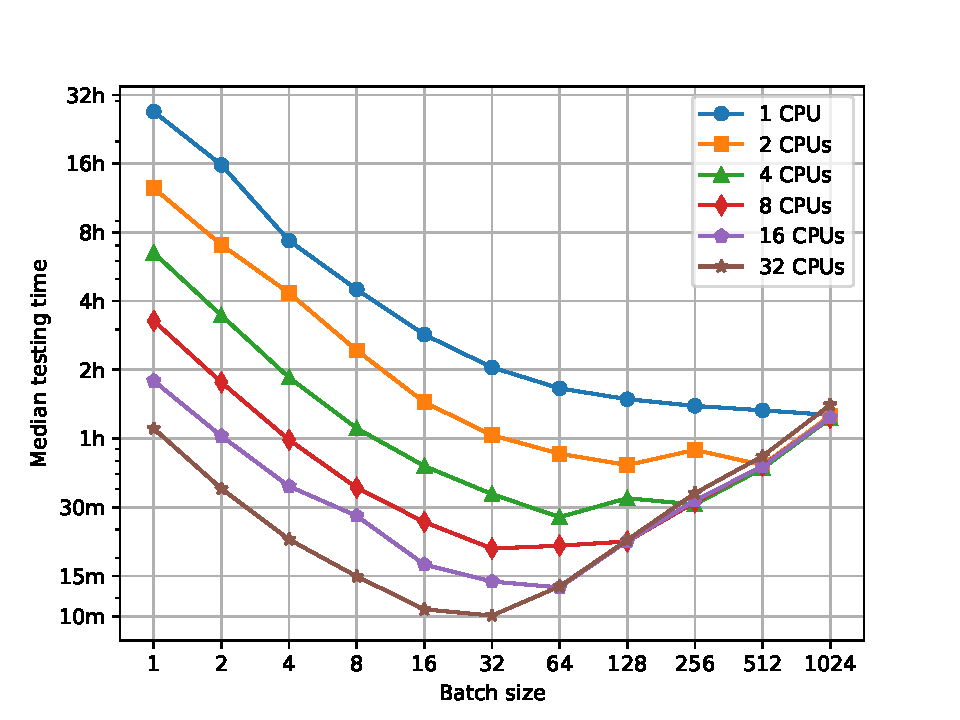
\includegraphics[trim={0.5cm 0.3cm 1.6cm 1.4cm}, clip, width=\linewidth]{images/speed-tests}
\caption{The median testing times for different numbers of \acro{CPU}s and batch sizes}
\label{fig:results}
\end{figure}

\section{Results}
\label{sec:results}

Figure~\ref{fig:results} shows the results of our experiments. In this section, we discuss the results and how they relate to the three research questions outlined in the previous section.

\subsection{Multiprocessing}
With batch size 1, the testing speed scales almost linearly with the number of \acro{CPU}s, as we would expect. Whereas with with 1~\acro{CPU}, the median testing time is 27~hours and 2~minutes, it is only 1~hour and 6~minutes with 32~\acro{CPU}s (about 24-fold speed-up).\footnote{%
The reason why we did not achieve the theoretical 32-fold speedup is likely due to tasks from other users on our server.%
}

\subsection{Batching of test files}
With 1~\acro{CPU}, the testing speed also scales almost linearly with the batch size up to a point. Whereas with batch size 1, the median testing time is 27~hours and 2~minutes, it is only 4~hours and 30~minutes with batch size 8 (about 6-fold speed-up), and only 1~hour and 20~minutes with batch size 512 (about 21-fold speed-up). This indicates that initialization dominates the testing time.

To better understand the relationship between the initialization and the testing time, we can solve the following series of equations:
\begin{align*}
    14\cdot(783\cdot(X + Y)) &= \text{27 hours and 2 minutes} \\
    14\cdot(X + 783\cdot Y) &= \text{1 hour and 16 minutes}
\end{align*}
On the left-hand side of the equations, the variable $X$ stands for the mean time that it takes to initialize a \TeX{} format and the variable $Y$ stands for the mean time that it takes to process the markdown text from a single test file. On the right-hand side of the equations are the median testing times with 1~\acro{CPU} and batch sizes 1 (above) and 1024 (below).

The solution shows that whereas it takes $X\approx\text{8.47 seconds}$ to initialize a \TeX{} format, it takes only $Y\approx\text{0.41 seconds}$ to process a markdown text. In other words, without batching, 95\% of time is spent on initialization and only 5\% on actual testing; with batching, up to 97\% of time is spent on actual testing.

\subsection{Batch size limiting}
The speed improvements from multiprocessing and batching are additive up to a point. Whereas with 1~\acro{CPU} and batch size 1, the median testing time is 27~hours and 2~minutes, it is only 10~minutes with 32~\acro{CPU}s and batch size 32 (about 161-fold speed-up).

When the number of \acro{CPU}s multiplied by the batch size exceeds the number of test files (783), we cannot use all \acro{CPU}s and the testing speed decreases. Whereas with 32~\acro{CPU}s and batch size 16, the median testing time is only 11~minutes, it is 1~hour and 24~minutes with the same number of \acro{CPU}s and batch size 1024 (about 8-fold slow-down). Our framework prevents this by limiting the batch size.

\section{Related work}
\label{sec:related-work}

In this section, we discuss prior work related to our framework.

\subsection{The l3build package}
The l3build package~\cite{mittelbach2014l3build, wright2015automating, wright2022l3build, latex2023l3build} provides a comprehensive system for \TeX{} package management that also includes a regression testing framework.

Unlike our framework, the l3build package is written in Lua, which has no built-in support for multiprocessing. Therefore, l3build needs external tools like \acro{GNU}~Parallel to use multiple \acro{CPU}s for testing.
\looseness=-1

In the Markdown package, each test file is designed to hold a single self-contained test that avoids modifying the global state. This design allows for straightforward grouping of tests into batches, where each test is isolated from others using \TeX{} groups, as we discussed in Section~\ref{sec:batching-of-test-files}.

In the l3build package, a single test file may contain multiple tests. These tests can be interdependent, creating a challenge in separating them from their respective files. Additionally, these tests might change the global state, which poses a risk of unexpected conflicts when tests are grouped into batches. Due to these complexities, the l3build package does not support the batching of test files. Nonetheless, the practice of including multiple tests in a single test file can be seen as a form of manual batching that amortizes the cost of initialization.

\subsection{Batching and batch splitting}
The techniques of batching and batch splitting were perhaps first used with \TeX{} in the ARQMath competitions for large-scale indexing of math formulae.

In the first ARQMath competition, the \acro{MIRMU} team used the \LaTeX ML tool to convert \TeX{} formulae to the \acro{XML} format~\cite[Section~2.2]{novotny2020three}. Due to speed issues when processing each formula separately, \acro{MIRMU} processed them in batches. However, a single error would cause the loss of an entire batch. Therefore, \acro{MIRMU} used batch splitting to recover correct formulae after an error.~\cite{novotny2020arqmath} The combination of batching and batch splitting allowed \acro{MIRMU} to convert the formulae quickly and losslessly.

\section{Conclusion}
\label{sec:conclusion}

Larger \TeX{} projects commonly use regression tests to ensure code integrity over time.
In this study, we explored techniques for speeding up the regression testing of \TeX{} packages. Using multiprocessing and the batching of test files, we improved the testing time of the Markdown package from hours to minutes.
\looseness=-1

Our techniques are general and can be used to speed up other testing frameworks for \TeX{} packages. This advancement is likely to streamline the development cycles for \TeX{} packages.

\medskip
\noindent
\input images/wolf-f1

\section*{Acknowledgements}
We would like to gratefully acknowledge the Natural Language Processing Center at the Faculty of Informatics, Masaryk University, Brno, who kindly provided computational resources for our experiments.

\bibliographystyle{tugboat}
\begingroup
\gappto{\UrlBreaks}{\UrlOrds}
\RaggedRight
\bibliography{main}
\endgroup

\makesignature
\end{document}
